\section{Proving that X25519 in Coq matches the mathematical model}
\label{sec:maths}

In this section we prove the following informal theorem:

\begin{informaltheorem}
  The implementation of X25519 in TweetNaCl computes the
  $\F{p}$-restricted \xcoord scalar multiplication on $E(\F{p^2})$ where $p$ is $\p$
  and $E$ is the elliptic curve $y^2 = x^3 + 486662 x^2 + x$.
\end{informaltheorem}

More precisely, we prove that our formalization of the RFC matches the definitions of Curve25519 by Bernstein:
\begin{lstlisting}[language=Coq]
Theorem RFC_Correct: forall (n p : list Z)
  (P:mc curve25519_Fp2_mcuType),
  Zlength n = 32 ->
  Zlength p = 32 ->
  Forall (fun x => 0 <= x /\ x < 2 ^ 8) n ->
  Forall (fun x => 0 <= x /\ x < 2 ^ 8) p ->
  Fp2_x (decodeUCoordinate p) = P#x0 ->
  RFC n p =
    encodeUCoordinate
      ((P *+ (Z.to_nat (decodeScalar25519 n))) _x0).
\end{lstlisting}

We first review the work of Bartzia and Strub \cite{BartziaS14} (\ref{subsec:ECC-Weierstrass}).
We extend it to support Montgomery curves (\ref{subsec:ECC-Montgomery})
with homogeneous coordinates (\ref{subsec:ECC-projective}) and prove the
correctness of the ladder (\ref{subsec:ECC-ladder}).
We discuss the twist of Curve25519 (\ref{subsec:Zmodp}) and explain how we deal
with it in the proofs (\ref{subsec:curvep2}).

\subsection{Formalization of elliptic Curves}
\label{subsec:ECC}

\fref{tikz:ProofHighLevel1} presents the structure of the proof of the ladder's
correctness.
\begin{figure}[h]
  \centering
  \begin{tikzpicture}[textstyle/.style={black, anchor= south west, align=center, minimum height=0.45cm, text centered, font=\tiny}]


  % Bartzia & Strub
  \draw[dashed, fill=doc@lstbackground] (2.75,0.5) -- (2.75,2) -- (6,2) -- (6, 0.5) -- cycle;
  \draw (6,2) node[textstyle, anchor=north east] {Library from Bartzia \& Strub};

  % Mab
  \begin{scope}[yshift=0 cm,xshift=0 cm]
    \draw (0,0) -- (1.5,0) -- (1.5,-0.75) -- (0, -0.75) -- cycle;
    \draw (0.75,-0.375) node[textstyle, anchor=center] {$M_{a,b}(\K)$};
  \end{scope}

  % Eab
  \begin{scope}[yshift=1.5 cm,xshift=3 cm]
    \draw[fill=white] (0,0) -- (1.5,0) -- (1.5,-0.75) -- (0, -0.75) -- cycle;
    \draw (0.75,-0.375) node[textstyle, anchor=center] {$E_{a',b'}(\K)$};
  \end{scope}

  % M is a finite assoc group
  \begin{scope}[yshift=0 cm,xshift=3 cm]
    \draw [fill=green!20] (0,0) -- (3.25,0) -- (3.25,-0.75) -- (0, -0.75) -- cycle;
    \draw (1.675,-0.375) node[textstyle, anchor=center] {$M_{a,b}(\K)$ is an abelian group};
  \end{scope}

  % Hypothesis x square is not 2
  \begin{scope}[yshift=-1.5 cm,xshift=0 cm]
    \draw [fill=orange!20] (0,0) -- (1.5,0) -- (1.5,-1.25) -- (0, -1.25) -- cycle;
    \draw (0,0) node[textstyle, anchor=north west] {\textbf{Hyp:}};
    \draw (0.75,-0.375) node[textstyle, anchor=north] {$\forall x \in \K,$\\[.6ex]$x^2 \neq a^2-4$};
  \end{scope}

  % Final theorem
  \begin{scope}[yshift=-1.5 cm,xshift=3 cm]
    \draw [fill=green!20] (0,0) -- (3.25,0) -- (3.25,-1.375) -- (0, -1.375) -- cycle;
    \draw (0,0) node[textstyle, anchor=north west] {\textbf{Thm:}};
    \draw (1.675,-0.375) node[textstyle, anchor=north] {$\forall x \in \K, n \in \N, P \in M_{a,b}(\K),$\\[.6ex]$x = \chi_0(P) \implies$\\[.6ex]ladder $n$ $x$ = $\chi_0(n \cdot P)$};
  \end{scope}

  \path [thick, double, ->] (1.5,-0.375) edge  [out=0, in=-180] (3,-0.375);
  \path [thick, double, ->] (3.75,0.75) edge  [out=-90, in=90] (3.75,0);
  \path [thick, double, ->] (3.75,-0.75) edge  [out=-90, in=90] (3.75,-1.5);
  \path [thick, double, ->] (1.5,-2.125) edge  [out=0, in=-180] (3,-2.125);


\end{tikzpicture}

  \caption{Overview of the proof of Montgomery ladder's correctness}
  \label{tikz:ProofHighLevel1}
\end{figure}

We consider elliptic curves over a field $\K$. We assume that the
characteristic of $\K$ is neither 2 or 3.

\begin{dfn}
  Given a field $\K$,
  using an appropriate choice of coordinates,
  an elliptic curve $E$
  is a plane cubic algebraic curve defined by an equation $E(x,y)$ of the form:
  $$E : y^2 + a_1 xy + a_3 y = x^3 + a_2 x^2 + a_4 x + a_6$$
  where the $a_i$'s are in \K\ and the curve has no singular point (\ie no cusps
  or self-intersections). The set of points defined over \K, written $E(\K)$, is formed by the
  solutions $(x,y)$ of $E$ together with a distinguished point $\Oinf$ called point at infinity:
  $$E(\K) = \{ (x,y) \in \K \times \K ~|~E(x,y)\} \cup \{\Oinf\}$$
\end{dfn}

\subsubsection{Short Weierstra{\ss} curves}
\label{subsec:ECC-Weierstrass}

This equation $E(x,y)$ can be reduced into its short Weierstra{\ss} form.

\begin{dfn}
  Let $a \in \K$ and $b \in \K$ such that $$\Delta(a,b) = -16(4a^3 + 27b^2) \neq 0.$$
  The \textit{elliptic curve} $E_{a,b}$ is defined by the equation:
  $$y^2 = x^3 + ax + b.$$
  $E_{a,b}(\K)$ is the set of all points $(x,y) \in \K^2$ satisfying the $E_{a,b}$
  along with an additional formal point $\Oinf$, ``at infinity''. Such a curve does not have any singularity.
\end{dfn}

In this setting, Bartzia and Strub defined the parametric type \texttt{ec} which
represent the points on a specific curve. It is parameterized by
a \texttt{K : ecuFieldType} --- the type of fields whose characteristic is not 2 or 3 ---
and \texttt{E : ecuType} --- a record that packs the curve parameters $a$ and $b$
along with the proof that $\Delta(a,b) \neq 0$.
\begin{lstlisting}[language=Coq]
Inductive point := EC_Inf | EC_In of K * K.
Notation "(| x, y |)" := (EC_In x y).
Notation "\infty" := (EC_Inf).

Record ecuType :=
  { A : K; B : K; _ : 4 * A^3 + 27 * B^2 != 0}.
Definition oncurve (p : point) :=
  if p is (| x, y |)
    then y^2 == x^3 + A * x + B
    else true.
Inductive ec : Type := EC p of oncurve p.
\end{lstlisting}

Points on an elliptic curve are equipped with the structure of an abelian group.
\begin{itemize}
  \item The negation of a point $P = (x,y)$ is defined by reflection over the $x$ axis $-P = (x, -y)$.
  \item The addition of two points $P$ and $Q$ is defined as the negation of the third intersection point
        of the line passing through $P$ and $Q$, or tangent to $P$ if $P = Q$.
  \item $\Oinf$ is the neutral element under this law: if 3 points are collinear, their sum is equal to $\Oinf$.
\end{itemize}
These operations are defined in Coq as follows (where we omit the code for the tangent case):
\begin{lstlisting}[language=Coq]
Definition neg (p : point) :=
  if p is (| x, y |) then (| x, -y |) else EC_Inf.

Definition add (p1 p2 : point) :=
  match p1, p2 with
    | \infty , _ => p2
    | _ , \infty => p1
    | (| x1, y1 |), (| x2, y2 |) =>
      if x1 == x2 then ... else
        let s := (y2 - y1) / (x2 - x1) in
        let xs := s^2 - x1 - x2 in
          (| xs, - s * (xs - x1 ) - y1 |)
  end.
\end{lstlisting}
The value of \texttt{add} is proven to be on the curve with coercion:
\begin{lstlisting}[language=Coq]
Lemma addO (p q : ec): oncurve (add p q).

Definition addec (p1 p2 : ec) : ec :=
  EC p1 p2 (addO p1 p2)
\end{lstlisting}

\subsubsection{Montgomery curves}
\label{subsec:ECC-Montgomery}

Speedups can be obtained by switching to homogeneous coordinates and other forms
than the Weierstra{\ss} form. We consider the Montgomery form \cite{MontgomerySpeeding}.

\begin{dfn}
  Let $a \in \K \backslash \{-2, 2\}$, and $b \in \K \backslash \{ 0\}$.
  The \textit{elliptic curve} $M_{a,b}$ is defined by the equation:
  $$by^2 = x^3 + ax^2 + x,$$
  $M_{a,b}(\K)$ is the set of all points $(x,y) \in \K^2$ satisfying the $M_{a,b}$
  along with an additional formal point $\Oinf$, ``at infinity''.
\end{dfn}
Similar to the definition of \texttt{ec}, we defined the parametric type \texttt{mc} which
represents the points on a specific Montgomery curve.
It is parameterized by
a \texttt{K : ecuFieldType} --- the type of fields whose characteristic is not
2 or 3 --- and \texttt{M : mcuType} --- a record that packs the curve
parameters $a$ and $b$ along with the proofs that $b \neq 0$ and $a^2 \neq 4$.
\begin{lstlisting}[language=Coq,belowskip=-0.1 \baselineskip]
Record mcuType :=
  { cA : K; cB : K; _ : cB != 0; _ : cA^2 != 4}.
Definition oncurve (p : point K) :=
if p is (| x, y |)
  then cB * y^+2 == x^+3 + cA * x^+2 + x
  else true.
Inductive mc : Type := MC p of oncurve p.

Lemma oncurve_mc: forall p : mc, oncurve p.
\end{lstlisting}
We define the addition on Montgomery curves in a similar way as for the Weierstra{\ss} form.
\begin{lstlisting}[language=Coq,belowskip=-0.25 \baselineskip]
Definition add (p1 p2 : point K) :=
  match p1, p2 with
    | \infty, _ => p2
    | _, \infty => p1
    | (|x1, y1|), (|x2, y2|) =>
      if   x1 == x2
      then if  (y1 == y2) && (y1 != 0)
           then ... else \infty
      else
        let s  := (y2 - y1) / (x2 - x1) in
        let xs := s^+2 * cB - cA - x1 - x2 in
          (| xs, - s * (xs - x1) - y1 |)
    end.
\end{lstlisting}
And again we prove the result is on the curve: % (again with coercion):
\begin{lstlisting}[language=Coq]
Lemma addO (p q : mc) : oncurve (add p q).
Definition addmc (p1 p2 : mc) : mc :=
  MC p1 p2 (addO p1 p2)
\end{lstlisting}

We then define a bijection between a Montgomery curve and its short Weierstra{\ss} form.
In this way we get associativity of addition on Montgomery curves from the
corresponding property for Weierstra{\ss} curves.
\begin{lemma}
  Let $M_{a,b}$ be a Montgomery curve, define
  $$a' = \frac{3-a^2}{3b^2} \text{\ \ \ \ and\ \ \ \ } b' = \frac{2a^3 - 9a}{27b^3}.$$
  then $E_{a',b'}$ is an elliptic curve, and the mapping
  $\varphi : M_{a,b} \mapsto E_{a',b'}$ defined as:
  \begin{align*}
    \varphi(\Oinf_M)   & = \Oinf_E                                                 \\
    \varphi( (x , y) ) & = \left( \frac{x}{b} + \frac{a}{3b} , \frac{y}{b} \right)
  \end{align*}
  is an isomorphism between elliptic curves.
\end{lemma}
\begin{lstlisting}[language=Coq,belowskip=-0.25 \baselineskip]
Definition ec_of_mc_point p :=
  match p with
  | \infty => \infty
  | (|x, y|) => (|x/(M#b) + (M#a)/(3%:R * (M#b)), y/(M#b)|)
  end.
Lemma ec_of_mc_point_ok p :
  oncurve M p ->
  ec.oncurve E (ec_of_mc_point p).

Definition ec_of_mc p :=
  EC (ec_of_mc_point_ok (oncurve_mc p)).

Lemma ec_of_mc_bij : bijective ec_of_mc.
\end{lstlisting}

\subsubsection{Projective coordinates}
\label{subsec:ECC-projective}

In a projective plane, points are represented with triples $(X:Y:Z)$,
with the exception of $(0:0:0)$.
Scalar multiples are representing the same point, \ie
for all $\lambda \neq 0$, the triples $(X:Y:Z)$ and $(\lambda X:\lambda Y:\lambda Z)$ represent
the same point.
For $Z\neq 0$, the projective point $(X:Y:Z)$ corresponds to the
point $(X/Z,Y/Z)$ on the affine plane. Likewise the point $(X,Y)$ on the
affine plane corresponds to $(X:Y:1)$ on the projective plane.

Using fractions as coordinates, the equation for a Montgomery curve $M_{a,b}$
becomes:
$$b \bigg(\frac{Y}{Z}\bigg)^2 = \bigg(\frac{X}{Z}\bigg)^3 + a \bigg(\frac{X}{Z}\bigg)^2 + \bigg(\frac{X}{Z}\bigg)$$
Multiplying both sides by $Z^3$ yields:
$$b Y^2Z = X^3 + a X^2Z + XZ^2$$
With this equation we can additionally represent the ``point at infinity''. By
setting $Z=0$, we derive $X=0$, giving us the ``infinite point'' $(0:1:0)$.

By restricting the parameter $a$ of $M_{a,b}(\K)$ such that $a^2-4$ is not a
square in \K, we ensure that $(0,0)$ is the only point with a $y$-coordinate of $0$.
\begin{hypothesis}
  \label{hyp:a_minus_4_not_square}
  $a^2-4$ is not a square in \K.
\end{hypothesis}
\begin{lstlisting}[language=Coq]
Hypothesis mcu_no_square : forall x : K, x^+2 != (M#a)^+2 - 4%:R.
\end{lstlisting}

We define $\chi$ and $\chi_0$ to return the \xcoord of points on a curve.
\begin{dfn}Let $\chi$ and $\chi_0$:\\
  -- $\chi : M_{a,b}(\K) \to \K \cup \{\infty\}$\\
  such that $\chi(\Oinf) = \infty$ and $\chi((x,y)) = x$.\\
  -- $\chi_0 : M_{a,b}(\K) \to \K$\\
  such that $\chi_0(\Oinf) = 0$ and $\chi_0((x,y)) = x$.
\end{dfn}
Using projective coordinates we prove the formula for differential addition.% (\lref{lemma:xADD}).
\begin{lemma}
  \label{lemma:xADD}
  Let $M_{a,b}$ be a Montgomery curve such that $a^2-4$ is not a square in \K, and
  let $X_1, Z_1, X_2, Z_2, X_4, Z_4 \in \K$, such that $(X_1,Z_1) \neq (0,0)$,
  $(X_2,Z_2) \neq (0,0)$, $X_4 \neq 0$ and $Z_4 \neq 0$.
  Define
  \begin{align*}
    X_3 & = Z_4((X_1 - Z_1)(X_2+Z_2) + (X_1+Z_1)(X_2-Z_2))^2  \\
    Z_3 & = X_4((X_1 - Z_1)(X_2+Z_2) - (X_1+Z_1)(X_2-Z_2))^2,
  \end{align*}
  then for any point $P_1$ and $P_2$ in $M_{a,b}(\K)$ such that
  $X_1/Z_1 = \chi(P_1), X_2/Z_2 = \chi(P_2)$, and $X_4/Z_4 = \chi(P_1 - P_2)$,
  we have $X_3/Z_3 = \chi(P_1+P_2)$.\\
  \textbf{Remark:}
  These definitions should be understood in $\K \cup \{\infty\}$.
  If $x\ne 0$ then we define $x/0 = \infty$.
\end{lemma}
Similarly we also prove the formula for point doubling.% (\lref{lemma:xDBL}).
\begin{lemma}
  \label{lemma:xDBL}
  Let $M_{a,b}$ be a Montgomery curve such that $a^2-4$ is not a square in \K, and
  let $X_1, Z_1 \in \K$, such that $(X_1,Z_1) \neq (0,0)$. Define
  \begin{align*}
    c   & = (X_1 + Z_1)^2 - (X_1 - Z_1)^2                   \\
    X_3 & = (X_1 + Z_1)^2(X_1-Z_1)^2                        \\
    Z_3 & = c\Big((X_1 + Z_1)^2+\frac{a-2}{4}\times c\Big),
  \end{align*}
  then for any point $P_1$ in $M_{a,b}(\K)$ such that $X_1/Z_1 = \chi(P_1)$,
  we have $X_3/Z_3 = \chi(2P_1)$.
\end{lemma}

With \lref{lemma:xADD} and \lref{lemma:xDBL}, we are able to compute efficiently
differential additions and point doublings using projective coordinates.

\subsubsection{Scalar multiplication algorithms}
\label{subsec:ECC-ladder}

By taking \aref{alg:montgomery-ladder} and replacing \texttt{xDBL\&ADD} by a
combination of the formulae from \lref{lemma:xADD} and \lref{lemma:xDBL},
we define a ladder \coqe{opt_montgomery} (in which $\K$ has not been fixed yet).
% similar to the one used in TweetNaCl (with \coqe{montgomery_rec}).
% shown above.

% We prove its correctness for any point whose \xcoord is not 0.
%
% \begin{lstlisting}[language=Coq,belowskip=-0.25 \baselineskip]
% Lemma opt_montgomery_x :
%   forall (n m : nat) (x : K),
%   n < 2^m -> x != 0 ->
%   forall (p : mc M), p#x0 = x ->
%   opt_montgomery n m x = (p *+ n)#x0.
% \end{lstlisting}
% We can remark that for an input $x = 0$, the ladder returns $0$.
% \begin{lstlisting}[language=Coq,belowskip=-0.25 \baselineskip]
% Lemma opt_montgomery_0:
%   forall (n m : nat), opt_montgomery n m 0 = 0.
% \end{lstlisting}
% Also \Oinf\ is the neutral element of $M_{a,b}(\K)$.
% \begin{lstlisting}[language=Coq,belowskip=-0.25 \baselineskip]
% Lemma p_x0_0_eq_0 : forall (n : nat) (p : mc M),
%   p #x0 = 0%:R -> (p *+ n) #x0 = 0%R.
% \end{lstlisting}
% This gives us the theorem of the correctness of the Montgomery ladder.

This gives us the theorem of the correctness of the Montgomery ladder.
\begin{theorem}
  \label{thm:montgomery-ladder-correct}
  For all $n, m \in \N$, $x \in \K$, $P \in M_{a,b}(\K)$,
  if $\chi_0(P) = x$ then \coqe{opt_montgomery} returns $\chi_0(n \cdot P)$
\end{theorem}
\begin{lstlisting}[language=Coq]
Theorem opt_montgomery_ok (n m: nat) (x : K) :
  n < 2^m ->
  forall (p : mc M), p#x0 = x ->
  opt_montgomery n m x = (p *+ n)#x0.
\end{lstlisting}
The definition of \coqe{opt_montgomery} is similar to \coqe{montgomery_rec_swap}
that was used in \coqe{RFC}.
We proved their equivalence, and used it in our
final proof of \coqe{Theorem RFC_Correct}.


\subsection{Curves, twists and extension fields}
\label{subsec:curve_twist_fields}

\fref{tikz:ProofHighLevel2} gives a high-level view of the proofs presented here.

\begin{figure}[h]
  \centering
  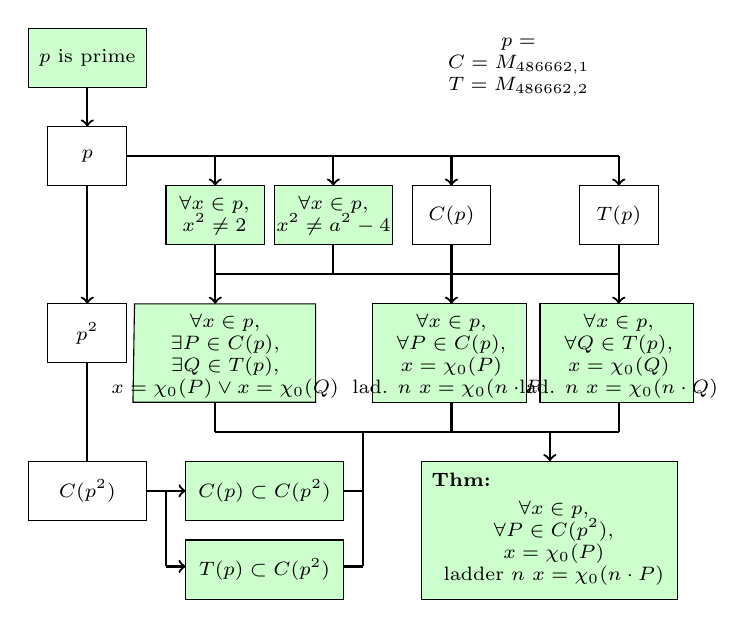
\begin{tikzpicture}[textstyle/.style={black, anchor= south west, align=center, minimum height=0.45cm, text centered, font=\scriptsize}]

  \draw (6.75,1) node[textstyle, anchor=north east] {$p = \p$\\$C = M_{486662,1}$\\$T = M_{486662,2}$\\};

  \begin{scope}[yshift=1 cm,xshift=-0.5 cm]
   \draw [fill=green!20] (0,0) -- (1.5,0) -- (1.5,-0.75) -- (0, -0.75) -- cycle;
   \draw (0.75,-0.375) node[textstyle, anchor=center] {$p$ is prime};
  \end{scope}

  \begin{scope}[yshift=-0.25 cm,xshift=-0.5 cm]
   \draw[fill=white] (0.25,0) -- (1.25,0) -- (1.25,-0.75) -- (0.25, -0.75) -- cycle;
   \draw (0.75,-0.375) node[textstyle, anchor=center] {$\F{p}$};
  \end{scope}

  \begin{scope}[yshift=-1 cm,xshift=1.25 cm]
   \draw[fill=green!20] (0,0) -- (1.25,0) -- (1.25,-0.75) -- (0, -0.75) -- cycle;
   \draw (0.615,-0.375) node[textstyle, anchor=center] {$\forall x \in \F{p},$\\$x^2 \neq 2$};
  \end{scope}

  \begin{scope}[yshift=-1 cm,xshift=2.625 cm]
   \draw[fill=green!20] (0,0) -- (1.5,0) -- (1.5,-0.75) -- (0, -0.75) -- cycle;
   \draw (0.75,-0.375) node[textstyle, anchor=center] {$\forall x \in \F{p},$\\$x^2 \neq a^2-4$};
  \end{scope}

  \begin{scope}[yshift=-1 cm,xshift=4.375 cm]
   \draw[fill=white] (0,0) -- (1,0) -- (1,-0.75) -- (0, -0.75) -- cycle;
   \draw (0.5,-0.375) node[textstyle, anchor=center] {$C(\F{p})$};
  \end{scope}

  \begin{scope}[yshift=-1 cm,xshift=6.5 cm]
   \draw[fill=white] (0,0) -- (1,0) -- (1,-0.75) -- (0, -0.75) -- cycle;
   \draw (0.5,-0.375) node[textstyle, anchor=center] {$T(\F{p})$};
  \end{scope}

  \path [thick, double, ->] (0.25,0.25) edge  [out=-90, in=90] (0.25,-0.25);
  \path [thick, double]     (0.75,-0.625) edge  [out=0, in=180] (7,-0.625);
  \path [thick, double, ->] (1.875,-0.625) edge  [out=-90, in=90] (1.875,-1);
  \path [thick, double, ->] (3.375,-0.625) edge  [out=-90, in=90] (3.375,-1);
  \path [thick, double, ->] (4.875,-0.625) edge  [out=-90, in=90] (4.875,-1);
  \path [thick, double, ->] (7,-0.625) edge  [out=-90, in=90] (7,-1);


  \begin{scope}[yshift=-2.5 cm,xshift=1.25 cm]
   \draw[fill=green!20] (-0.40,0) -- (1.90,0) -- (1.90,-1.25) -- (-0.42, -1.25) -- cycle;
   \draw (0.75,0) node[textstyle, anchor=north] {$\forall x \in \F{p},$\\$\exists P \in C(\F{p}),$\\$\exists Q \in T(\F{p})$,\\$x = \chi_0(P)\vee x = \chi_0(Q)$};
  \end{scope}

  \begin{scope}[yshift=-2.5 cm,xshift=4.125 cm]
   \draw[fill=green!20] (-0.25,0) -- (1.70,0) -- (1.70,-1.25) -- (-0.25, -1.25) -- cycle;
   \draw (0.75,0) node[textstyle, anchor=north] {$\forall x \in \F{p},$\\$\forall P \in C(\F{p}),$\\$x = \chi_0(P)\implies$\\lad. $n$ $x = \chi_0(n \cdot P)$};
  \end{scope}

  \begin{scope}[yshift=-2.5 cm,xshift=6.25 cm]
   \draw[fill=green!20] (-0.25,0) -- (1.70,0) -- (1.70,-1.25) -- (-0.25, -1.25) -- cycle;
   \draw (0.75,0) node[textstyle, anchor=north] {$\forall x \in \F{p},$\\$\forall Q \in T(\F{p}),$\\$x = \chi_0(Q)\implies$\\lad. $n$ $x = \chi_0(n \cdot Q)$};
  \end{scope}

  \path [thick, double, ->] (1.875,-1.75) edge  [out=-90, in=90] (1.875,-2.5);
  \path [thick, double]     (1.875,-2.125) edge  [out=0, in=180] (7,-2.125);
  \path [thick, double]     (3.375,-1.75) edge  [out=-90, in=90] (3.375,-2.125);
  \path [thick, double, ->] (4.875,-1.75) edge  [out=-90, in=90] (4.875,-2.5);
  \path [thick, double, ->] (7,-1.75) edge  [out=-90, in=90] (7,-2.5);

% F(p^2)

  \path [thick, double, ->] (0.25,-1) edge  [out=-90, in=90] (0.25,-2.5);

  \begin{scope}[yshift=-2.5 cm,xshift=-0.5 cm]
    \draw[fill=white] (0.25,0) -- (1.25,0) -- (1.25,-0.75) -- (0.25, -0.75) -- cycle;
   \draw (0.75,-0.375) node[textstyle, anchor=center] {$\F{p^2}$};
  \end{scope}

  \path [thick, double, ->] (0.25,-3.25) edge  [out=-90, in=90] (0.25,-5);

  % C(F(p^2))

  \begin{scope}[yshift=-4.5 cm,xshift=-0.5 cm]
   \draw[fill=white] (0,0) -- (1.5,0) -- (1.5,-0.75) -- (0, -0.75) -- cycle;
   \draw (0.75,-0.375) node[textstyle, anchor=center] {$C(\F{p^2})$};
  \end{scope}

  \begin{scope}[yshift=-4.5 cm,xshift=1.5 cm]
   \draw[fill=green!20] (0,0) -- (2,0) -- (2,-0.75) -- (0, -0.75) -- cycle;
   \draw (1,-0.375) node[textstyle, anchor=center] {$C(\F{p}) \subset C(\F{p^2})$};
  \end{scope}

  \begin{scope}[yshift=-5.5 cm,xshift=1.5 cm]
   \draw[fill=green!20] (0,0) -- (2,0) -- (2,-0.75) -- (0, -0.75) -- cycle;
   \draw (1,-0.375) node[textstyle, anchor=center] {$T(\F{p}) \subset C(\F{p^2})$};
  \end{scope}

  \path [thick, double, ->] (1,-4.875) edge [out=0, in=-180] (1.5,-4.875);
  \path [thick, double] (1.25,-4.875) edge [out=-90, in=90] (1.25,-5.835);
  \path [thick, double, ->] (1.25,-5.835) edge [out=0, in=-180] (1.5,-5.835);

  \begin{scope}[yshift=-4.5 cm,xshift=4.5 cm]
    \draw [fill=green!20] (0,0) -- (3.25,0) -- (3.25,-1.75) -- (0, -1.75) -- cycle;
    \draw (0,0) node[textstyle, anchor=north west] {\textbf{Thm:}};
    \draw (1.675,-0.375) node[textstyle, anchor=north] {$\forall x \in \F{p},$\\$\forall P \in C(\F{p^2}),$\\$x = \chi_0(P)\implies$\\ladder $n$ $x = \chi_0(n \cdot P)$};
  \end{scope}

  \path [thick, double]     (1.875,-4.125) edge  [out=0, in=180] (7,-4.125);
  \path [thick, double]     (1.875,-3.75) edge  [out=-90, in=90] (1.875,-4.125);
  \path [thick, double]     (4.875,-3.75) edge  [out=-90, in=90] (4.875,-4.125);
  \path [thick, double]     (7,-3.75) edge  [out=-90, in=90] (7,-4.125);

  \path [thick, double]     (3.5,-4.875) edge  [out=0, in=180] (3.75,-4.875);
  \path [thick, double]     (3.5,-5.835) edge  [out=0, in=180] (3.75,-5.835);
  \path [thick, double]     (3.75,-5.835) edge  [out=90, in=-90] (3.75,-4.125);

  \path [thick, double, ->] (6.125,-4.125) edge [out=-90, in=90] (6.125,-4.5);

\end{tikzpicture}

  \caption{Proof dependencies for the correctness of X25519.}
  \label{tikz:ProofHighLevel2}
\end{figure}

To be able to use the \tref{thm:montgomery-ladder-correct} we need to satisfy
hypothesis~\ref{hyp:a_minus_4_not_square}:%
% $a^2-4$ is not a square in \K:
$$\forall x \in \K,\ x^2 \neq a^2-4.$$
However there always exists $x \in \F{p^2}$ such that $x^2 = a^2-4$,
preventing the use \tref{thm:montgomery-ladder-correct}
with $\K = \F{p^2}$.

\begin{sloppypar}
  We first study Curve25519 and one of its quadratic twists Twist25519,
  both defined over \F{p}.
\end{sloppypar}

\subsubsection{Curves and twists}
\label{subsec:Zmodp}

We define $\F{p}$ as the numbers between $0$ and $p = \p$.
We create a \coqe{Zmodp} module to encapsulate those definitions.
\begin{lstlisting}[language=Coq]
Module Zmodp.
Definition betweenb x y z := (x <=? z) && (z <? y).
Definition p := locked (2^255 - 19).
Fact Hp_gt0 : p > 0.
Inductive type := Zmodp x of betweenb 0 p x.

Lemma Z_mod_betweenb (x y : Z) :
  y > 0 -> betweenb 0 y (x mod y).
Definition pi (x : Z) : type :=
  Zmodp (Z_mod_betweenb x Hp_gt0).
Coercion repr (x : type) : Z :=
  let: @Zmodp x _ := x in x.
\end{lstlisting}

We define the basic operations ($+, -, \times$) with their respective neutral
elements ($0, 1$) and prove \lref{lemma:Zmodp_field}.
\begin{lemma}
  \label{lemma:Zmodp_field}
  $\F{p}$ is a field.
\end{lemma}
For $a = 486662$, by using the Legendre symbol we prove that
$a^2 - 4$ and $2$ are not squares in $\F{p}$.
\begin{lstlisting}[language=Coq,belowskip=-0.25 \baselineskip]
Fact a_not_square : forall x: Zmodp.type,
  x^+2 != (Zmodp.pi 486662)^+2 - 4%:R.
\end{lstlisting}
\begin{lstlisting}[language=Coq,label=two_not_square,belowskip=-0.1 \baselineskip]
Fact two_not_square : forall x: Zmodp.type,
  x^+2 != 2%:R.
\end{lstlisting}
We now consider $M_{486662,1}(\F{p})$ and $M_{486662,2}(\F{p})$, one of its quadratic twists.
% \begin{dfn}Let the following instantiations of \aref{alg:montgomery-double-add}:\\
\begin{dfn}
  %Let the following instantiations of \aref{alg:montgomery-ladder}:\\
  We instantiate \coqe{opt_montgomery} in two specific ways:\\
  -- $Curve25519\_Fp(n,x)$ for $M_{486662,1}(\F{p})$.\\
  -- $Twist25519\_Fp(n,x)$ for $M_{486662,2}(\F{p})$.
\end{dfn}

With \tref{thm:montgomery-ladder-correct} we derive the following two lemmas:
\begin{lemma}
  For all $x \in \F{p},\ n \in \N,\ P \in \F{p} \times \F{p}$,\\
  such that $P \in M_{486662,1}(\F{p})$ and $\chi_0(P) = x$.
  $$Curve25519\_Fp(n,x) = \chi_0(n \cdot P)$$
\end{lemma}
\begin{lemma}
  For all $x \in \F{p},\ n \in \N,\ P \in \F{p} \times \F{p}$\\
  such that $P \in M_{486662,2}(\F{p})$ and $\chi_0(P) = x$.
  $$Twist25519\_Fp(n,x) = \chi_0(n \cdot P)$$
\end{lemma}
As the Montgomery ladder does not depend on $b$, it is trivial to
see that the computations done for points in $M_{486662,1}(\F{p})$ and in
$M_{486662,2}(\F{p})$ are the same.
\begin{lstlisting}[language=Coq]
Theorem curve_twist_eq: forall n x,
  curve25519_Fp_ladder n x = twist25519_Fp_ladder n x.
\end{lstlisting}

Because $2$ is not a square in $\F{p}$, it allows us split $\F{p}$ into two sets.
\begin{lemma}
  \label{lemma:square-or-2square}
  For all $x$ in $\F{p}$, there exists $y$ in $\F{p}$ such that
  $$y^2 = x\ \ \ \lor\ \ 2y^2 = x$$
\end{lemma}
For all $x \in \F{p}$, we can compute $x^3 + ax^2 + x$. Using \lref{lemma:square-or-2square}
we can find a $y$ such that $(x,y)$ is either on the curve or on the quadratic twist:
\begin{lemma}
  \label{lemma:curve-or-twist}
  For all $x \in \F{p}$, there exists a point $P$ in $M_{486662,1}(\F{p})$ or
  in $M_{486662,2}(\F{p})$ such that the \xcoord of $P$ is $x$.
\end{lemma}
\begin{lstlisting}[language=Coq,belowskip=-0.5 \baselineskip]
Theorem x_is_on_curve_or_twist:
  forall x : Zmodp.type,
  (exists (p : mc curve25519_mcuType), p#x0 = x) \/
  (exists (p' : mc twist25519_mcuType), p'#x0 = x).
\end{lstlisting}

\subsubsection{Curve25519 over \F{p^2}}
\label{subsec:curvep2}

The quadratic extension $\F{p^2}$ is defined as $\F{p}[\sqrt{2}]$ by~\cite{Ber06}.
The theory of finite fields already has been formalized in the Mathematical Components
library,
%ref?
but this formalization is rather abstract, and we need concrete representations of field
elements here.
For this reason we decided to formalize a definition of $\F{p^2}$ ourselves.

We can represent $\F{p^2}$ as the set $\F{p} \times \F{p}$,
% in other words,
representing polynomials with coefficients in $\F{p}$ modulo $X^2 - 2$. In a similar way
as for $\F{p}$ we use a module in Coq.
\begin{lstlisting}[language=Coq,belowskip=-0.25 \baselineskip]
Module Zmodp2.
Inductive type :=
  Zmodp2 (x: Zmodp.type) (y:Zmodp.type).

Definition pi (x: Zmodp.type * Zmodp.type) : type :=
  Zmodp2 x.1 x.2.
Coercion repr (x: type) : Zmodp.type*Zmodp.type :=
  let: Zmodp2 u v := x in (u, v).
Definition mul (x y: type) : type :=
  pi ((x.1 * y.1) + (2%:R * (x.2 * y.2)),
      (x.1 * y.2) + (x.2 * y.1)).
\end{lstlisting}
% Definition zero : type :=
%   pi ( 0%:R, 0%:R ).
% Definition one : type :=
%   pi ( 1, 0%:R ).
% Definition opp (x: type) : type :=
%   pi (- x.1 , - x.2).
% Definition add (x y: type) : type :=
%   pi (x.1 + y.1, x.2 + y.2).
% Definition sub (x y: type) : type :=
%   pi (x.1 - y.1, x.2 - y.2).

We define the basic operations ($+, -, \times$) with their respective neutral
elements $0$ and $1$. Additionally we verify that for each element of in
$\F{p^2}\backslash\{0\}$, there exists a multiplicative inverse.
\begin{lemma}
  \label{lemma:Zmodp2_inv}
  For all $x \in \F{p^2}\backslash\{0\}$ and $a,b \in \F{p}$ such that $x = (a,b)$,
  $$x^{-1} = \Big(\frac{a}{a^2-2b^2}\ , \frac{-b}{a^2-2b^2}\Big)$$
\end{lemma}
As in $\F{p}$, we define $0^{-1} = 0$ and prove \lref{lemma:Zmodp2_field}.
\begin{lemma}
  \label{lemma:Zmodp2_field}
  $\F{p^2}$ is a commutative field.
\end{lemma}

%% TOO LONG
%% If need remove this paragraph
We then specialize the basic operations in order to speed up the verification
of formulas by using rewrite rules:
\begin{equation*}
  \begin{split}
    (a,0) + (b,0) &= (a+b, 0)\\
    (a, 0)^{-1} &= (a^{-1}, 0)
  \end{split}
  \qquad
  \begin{split}
    (a,0) \cdot   (b,0) &= (a \cdot b, 0)\\
    (0,a)^{-1} &= (0,(2\cdot a)^{-1})
  \end{split}
\end{equation*}

The injection $a \mapsto (a,0)$ from $\F{p}$ to $\F{p^2}$ preserves
$0, 1, +, -, \times$. Thus $(a,0)$ can be abbreviated as $a$ without confusions.

We define $M_{486662,1}(\F{p^2})$. With the rewrite rule above, it is straightforward
to prove that any point on the curve $M_{486662,1}(\F{p})$ is also on the curve
$M_{486662,1}(\F{p^2})$. Similarly, any point on the quadratic twist
$M_{486662,2}(\F{p})$ also corresponds to a point on the curve $M_{486662,1}(\F{p^2})$.
As direct consequence, using \lref{lemma:curve-or-twist}, we prove that for all
$x \in \F{p}$, there exists a point $P \in \F{p^2}\times\F{p^2}$ on
$M_{486662,1}(\F{p^2})$ such that $\chi_0(P) = (x,0) = x$.

\begin{lstlisting}[language=Coq,belowskip=-0.25 \baselineskip]
Lemma x_is_on_curve_or_twist_implies_x_in_Fp2:
  forall (x:Zmodp.type),
    exists (p: mc curve25519_Fp2_mcuType),
      p#x0 = Zmodp2.Zmodp2 x 0.
\end{lstlisting}

We now study the case of the scalar multiplication and show similar proofs.
\begin{dfn}
  Define the functions $\varphi_c$, $\varphi_t$ and $\psi$\\
  -- $\varphi_c: M_{486662,1}(\F{p}) \mapsto M_{486662,1}(\F{p^2})$\\
  such that $\varphi((x,y)) = ((x,0), (y,0))$.\\
  -- $\varphi_t: M_{486662,2}(\F{p}) \mapsto M_{486662,1}(\F{p^2})$\\
  such that $\varphi((x,y)) = ((x,0), (0,y))$.\\
  -- $\psi: \F{p^2} \mapsto \F{p}$\\
  such that $\psi(x,y) = x$.
\end{dfn}

\begin{lemma}
  \label{lemma:proj}
  For all $n \in \N$, for all point $P\in\F{p}\times\F{p}$ on the curve
  $M_{486662,1}(\F{p})$ (respectively on the quadratic twist $M_{486662,2}(\F{p})$), we have:
  \begin{align*}
    P \in M_{486662,1}(\F{p}) & \implies \varphi_c(n \cdot P) = n \cdot \varphi_c(P) \\
    P \in M_{486662,2}(\F{p}) & \implies \varphi_t(n \cdot P) = n \cdot \varphi_t(P)
  \end{align*}
\end{lemma}
Notice that:
\begin{align*}
  \forall P \in M_{486662,1}(\F{p}),\ \ \psi(\chi_0(\varphi_c(P))) = \chi_0(P) \\
  \forall P \in M_{486662,2}(\F{p}),\ \ \psi(\chi_0(\varphi_t(P))) = \chi_0(P)
\end{align*}

In summary for all $n \in \N,\ n < 2^{255}$, for any given point $P\in\F{p}\times\F{p}$
in $M_{486662,1}(\F{p})$ or $M_{486662,2}(\F{p})$, $Curve25519\_Fp$
computes the $\chi_0(n \cdot P)$.
We proved that for all $P \in \F{p^2}\times\F{p^2}$ such that $\chi_0(P) \in \F{p}$
there exists a corresponding point on the curve or the twist over $\F{p}$.
We proved that for any point, on the curve or the twist we can compute the
scalar multiplication by $n$ and yield to the same result as if we did the
computation in $\F{p^2}$.
% As a result we have proved theorem 2.1 of \cite{Ber06}:
% No: missing uniqueness !
\begin{theorem}
  \label{thm:general-scalarmult}
  For all $n \in \N$, such that $n < 2^{255}$,
  for all $x \in \F{p}$ and $P \in M_{486662,1}(\F{p^2})$ such that $\chi_0(P) = x$,
  $Curve25519\_Fp(n,x)$ computes $\chi_0(n \cdot P)$.
\end{theorem}
which is formalized in Coq as:
\begin{lstlisting}[language=Coq,belowskip=-0.1 \baselineskip]
Theorem curve25519_Fp2_ladder_ok:
  forall (n : nat) (x:Zmodp.type),
  (n < 2^255)%nat ->
  forall (p  : mc curve25519_Fp2_mcuType),
  p #x0 = Zmodp2.Zmodp2 x 0 ->
  curve25519_Fp_ladder n x = (p *+ n)#x0 /p.
\end{lstlisting}

We then prove the equivalence between of operations in $\Ffield$ and $\Zfield$,
in other words between \coqe{Zmodp} and \coqe{:GF}.
This allows us to show that given a clamped value $n$ and normalized \xcoord of $P$,
\coqe{RFC} gives the same results as $Curve25519\_Fp$.

All put together, this finishes the proof of the mathematical correctness of X25519: the fact that the code in X25519, both in the RFC~7748 and
in TweetNaCl versions, correctly computes multiplication in the elliptic curve.
